\documentclass[a4paper,10pt]{article}

% Hier die Nummer des Blatts und Autoren angeben.
\newcommand{\blatt}{7}
\newcommand{\autor}{Till Schander (6682565)}

\usepackage{hci}

\begin{document}
% Seitenkopf mit Informationen
\kopf
\renewcommand{\figurename}{Abbildung}

\aufgabe{10}

\begin{figure}[ht]
\centering 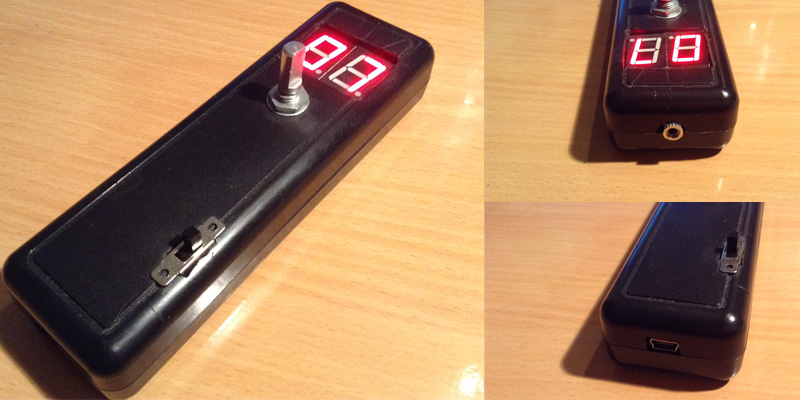
\includegraphics[width=1.0\textwidth]{intervalometer.jpg}
\caption{Das Intervalometer}
\end{figure}

Im folgenden wird ein Intervalometer anhand von fünf Gestaltungskriterien bewertet. Ich habe dieses Gerät vor einem halben Jahr gebaut, da ich Zeitrafferaufnahmen machen wollte, die Software meiner Kamera hierfür jedoch keine Option anbot. Am unteren rechten Rand ist ein Schiebeschalter zum Ein- und Ausschalten des Intervalometers. Mit dem Drehknopf in der oberen Mitte kann eingestellt werden, in welchen Abständen ein Foto gemacht werden soll. Beim Drehen wird der aktuell ausgewählte Abstand auf den zwei Siebensegmentanzeigen angezeigt. Die Zahl steht für die Sekunden zwischen jedem Foto. Wird die 99 überschritten, leuchtet zusätzlich ein Punkt auf. Ein Abstand wird ausgewählt, indem der Drehknopf heruntergedrückt wird. Dann blinkt die Anzeige um dem Nutzer zu signalisieren, dass nun die Fotos gemacht werden. Die Verbindung zur Kamera wird über ein Kabel mit 2,5mm Klinkenanschluss hergestellt. Dieses kann an der oberen Seite eingesteckt werden. An der unteren Seite befindet sich ein Mini-USB Anschluss, über den ggf. Softwareupdates auf den Mikrocontroller im inneren des Gehäuses geladen werden können. Das Intervalometer wird mit zwei AAA-Batterien betrieben. Um diese auszuwechseln muss das Gehäuse aufgeschraubt werden.

\subsection*{Funktionalität}
Da die Instrumente des Intervalometers gering in ihrer Zahl sind, ist die Funktionalität eines jeden Instruments schnell durchschaut. Die beiden Anschlüsse sind an den oberen und unteren Seiten. Dies ist zum einen, da sie am wenigsten von allen Instrumenten genutzt werden müssen. Außerdem werden hier Kabel eingesteckt, was eine Platzierung an der Unterseite umständlich machen würde. Auch auf der Oberseite könnten die Kabel die Nutzung der anderen Instrumente erschweren. Die beiden kürzeren Seiten machen das Auffinden der kleinen Anschlüsse schneller, als an der größeren Seiten. Da der Drehknopf sehr schmal ist, kann er kaum aus versehen bedient werden. Nach der Auswahl eines Intervalls kann dieses nicht mehr verändert werden, was ebenfalls unbeabsichtigte Änderungen verhindert. Der An- und Ausschalter ist leider etwas zu groß, weswegen er hingegen schon möglicherweise aus Versehen betätigt werden könnte. Das wechseln der Batterien ist sehr umständlich, da hierfür das Gehäuse aufgeschraubt werden muss. Glücklicherweise muss dies nicht häufig getan werden, da das Intervalometer nach der Auswahl eines Intervalls sein Display ausschaltet und so sehr stromsparend ist.

\subsection*{Ergonomie}
In seiner länglichen, schmalen Form liegt das Intervalometer gut in der Hand. Die Abgerundeten Ecken und Kanten helfen hier zusätzlich. Der Drehknopf ist lang genug um auch von großen Händen bedient werden zu können. Er ist lediglich ein wenig zu dünn. Das Display ist so groß, dass es auch von einiger Distanz noch sichtbar ist. Das Intervalometer kann auch im Dunkeln verwendet werden, da das Display leuchtet, und der Drehknopf bei jedem Schritt einrastet. Alle Instrumente sind weit genug auseinander, sodass beim Bedienen keins den anderen im weg ist. Da das Gerät sofort nach dem Einschalten benutzbar ist, ist es auch sehr effizient.

\subsection*{Ästhetik}
Das Intervalometer sieht relativ ansprechend aus. Bis auf der den An- und Ausschalter sind alle Instrumente mittig angeordnet. Dieser liegt auf einer Einkerbung im oberen Gehäuseteil und ist genauso weit von dem unteren Rand entfernt, wie der Drehknopf vom oberen Rand. Unterhalb des Drehknopfes ist eine große leere Fläche, welche mit dem oberen Bereich im Kontrast steht. Zusammen unterteilen sie das Intervalometer ungefähr im goldenen Schnitt. Die Anschlüsse sind exakt in der Mitte ihrer jeweiligen Seite platziert. Farblich ist das Gerät sehr Stilvoll in nur zwei Farben getönt. Das Gehäuse ist schwarz und die Instrumente sind silbern. Nach dem Einschalten kommt noch das rote Leuchten des Displays hinzu.

Weniger ansprechend ist, dass das Display nicht exakt mit dem Gehäuse abschließt. Der An- und Ausschalter hat außerdem zwei Löcher, welche zur Befestigung des Schalter genutzt werden können, hier jedoch schweben sie einfach ungenutzt über dem Gehäuse. Insgesamt folgt hier jedoch jedes Element dem Prinzip "form follows function". Es gibt bis auf die Kante auf der oberen Gehäusehälfte keinerlei unnötige Zierelemente.

\subsection*{Erlebnishaftigkeit}
An sich ist das Intervalometer wenig erlebnisorientiert, schließlich ist es eine kleine Box mit nur wenigen Instrumenten. Diese funktionieren jedoch genau so wie es zu erwarten wäre, weswegen zumindest kein Frust aufkommt. Die beiden Schalter ragen weit aus der Box heraus und laden so zum Benutzen ein. Das Betätigen des Drehknopf ist sehr befriedigend, da er sich nicht zu schwer dreht, jedoch trotzdem genügend Widerstand bietet. Da die Zahlen hell leuchten, ziehen sie den Nutzer zusätzlich in den Bann. Das Blinken dieser nach der Auswahl eines Intervalls ist zusätzlich unterhaltend.

\subsection*{Symbolik}
Einem Geschulten Anwender wird auffallen, dass das Intervalometer nicht industriell hergestellt wird. Menschen, die Vorlieben für DIY haben, werden daher dieses Gerät lieben. Beim Batterieauswechseln kann die Elektronik des Intervalometers betrachtet werden, was diese Personengruppe vermutlich interessieren wird. Für andere kann das Gerät mangels perfekter Verarbeitung billig und somit abstoßend wirken.

\end{document}
